\documentclass[border=3pt,tikz]{standalone}
\usepackage{newtxtext}
\usepackage{newtxmath}
\usetikzlibrary{positioning,arrows.meta,calc,fit,backgrounds}

\definecolor{OIskyblue}{HTML}{56B4E9}
\definecolor{OIblue}{HTML}{0072B2}
\definecolor{OIvermillion}{HTML}{D55E00}
\definecolor{OIorange}{HTML}{E69F00}
\definecolor{OIgreen}{HTML}{009E73}

\begin{document}
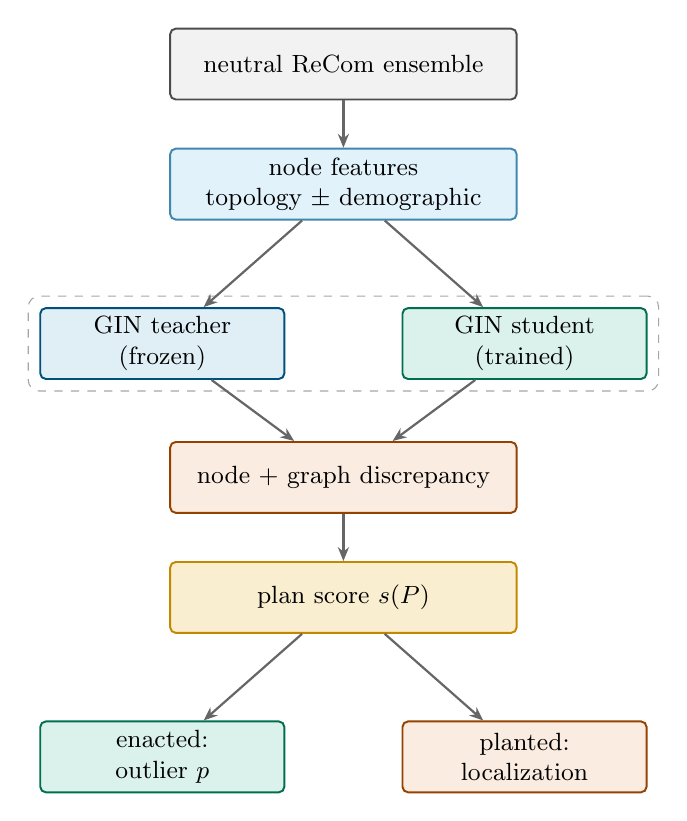
\begin{tikzpicture}[>=Stealth,
  block/.style={rectangle, rounded corners=2pt, draw=black!70, line width=0.7pt,
    minimum width=44mm, minimum height=9mm, inner sep=3pt, align=center, font=\small},
  half/.style={minimum width=31mm},
  arrow/.style={-{Stealth[length=5pt,width=4pt]}, line width=0.8pt, draw=black!60},
  groupbox/.style={draw=black!35, dashed, rounded corners=4pt, inner xsep=4pt, inner ysep=4pt}]

  \node[block, fill=black!5] (input) {neutral ReCom ensemble};
  \node[block, fill=OIskyblue!18, draw=OIskyblue!75!black, below=6mm of input]
    (feat) {node features\\topology $\pm$ demographic};
  \node[block, half, fill=OIblue!12, draw=OIblue!70!black, below=11mm of feat, xshift=-23mm]
    (teach) {GIN teacher\\(frozen)};
  \node[block, half, fill=OIgreen!14, draw=OIgreen!70!black, below=11mm of feat, xshift=23mm]
    (stud) {GIN student\\(trained)};
  \node[block, fill=OIvermillion!12, draw=OIvermillion!70!black, below=28mm of feat]
    (disc) {node $+$ graph discrepancy};
  \node[block, fill=OIorange!18, draw=OIorange!85!black, below=6mm of disc]
    (score) {plan score $s(P)$};
  \node[block, half, fill=OIgreen!14, draw=OIgreen!70!black, below=11mm of score, xshift=-23mm]
    (enact) {enacted:\\outlier $p$};
  \node[block, half, fill=OIvermillion!12, draw=OIvermillion!70!black, below=11mm of score, xshift=23mm]
    (plant) {planted:\\localization};

  \begin{pgfonlayer}{background}
    \node[groupbox, fit=(teach)(stud)] {};
  \end{pgfonlayer}

  \draw[arrow] (input) -- (feat);
  \draw[arrow] (feat) -- (teach);
  \draw[arrow] (feat) -- (stud);
  \draw[arrow] (teach) -- (disc);
  \draw[arrow] (stud) -- (disc);
  \draw[arrow] (disc) -- (score);
  \draw[arrow] (score) -- (enact);
  \draw[arrow] (score) -- (plant);
\end{tikzpicture}
\end{document}
